% double check \Theta calculations -- is the whole thing off by a factor of 2???
% error bars on dS values from a single fit


% add mention about Fig 2d by rewording this sentence: 
%"Although the extracted  can b e converted to gate-voltage-per-temperature units using a value for 
%  measured separately (right axis of Fig. 2e), the entropy itself, S , is determined directly from the 
%  t to dg_sens without any additional calibration, and without knowing the precise value of  T_res"

% mention QPC heater in text when discussing Fig 2a -- define I_{heat} in here 
% add equation and citation for fit in Fig 2d to caption
% remove _{res} subscripts from temps
% peak height --> "an added scaling parameter (dS(B=0))" when describing dS vs B fits

\documentclass[twocolumn,showpacs,amsmath,amssymb,prl,aps,superscriptaddress]{revtex4-1}

\usepackage{graphicx}
\usepackage{amsmath}
\usepackage{siunitx}
\usepackage{hyperref}

\begin{document}

\title{Direct Entropy Measurement in a Mesoscopic Quantum System}
\author{Nikolaus Hartman}
\email{nik.hartman@gmail.com}
\thanks{The raw data and Python code used for all figures and analysis can be found at \url{https://github.com/nikhartman/spin_entropy}}
\affiliation{University of British Columbia, Vancouver, BC, Canada}
\author{Saeed Fallahi}
\affiliation{Purdue University, Lafayette, IN, USA}
\author{Geoffrey C. Gardner}
\affiliation{Purdue University, Lafayette, IN, USA}
\author{Christian Olsen}
\affiliation{University of British Columbia, Vancouver, BC, Canada}
\author{Silvia Folk}
\affiliation{University of British Columbia, Vancouver, BC, Canada}
\author{Mohammad Samani}
\altaffiliation{The Hospital for Sick Children, Toronto, ON, Canada}
\altaffiliation{Fields Institute for Research in Mathematical Sciences, Toronto, ON, Canada}
\affiliation{University of British Columbia, Vancouver, BC, Canada}
\author{Michael Manfra}
\affiliation{Purdue University, Lafayette, IN, USA}
\author{Joshua Folk}
\affiliation{University of British Columbia, Vancouver, BC, Canada}
\date{\today}

%\begin{abstract}
%
%Measuring the entropy of an electronic state is a powerful tool for identifying its underlying microscopic character.  Such measurements are typically based on bulk properties, such as heat capacity, that are straightforward to observe in macroscopic samples but exceedingly difficult to access in mesoscopic systems that may consist of just a few electrons. Taking advantage of a well-known Maxwell relation, we realize a protocol for entropy-to-charge conversation in a gate-defined GaAs quantum dot that enables an entropy measurement of the first three quantum states in to the dot. The entropy of a single spin ($k_B \ln{2}$) is measured within 8\% accuracy, as is the entropy arising at the magnetic field-driven singlet-triplet crossing for two electrons.
%
%\end{abstract}

\maketitle

%%%%%%% intro material %%%%%%%%%
\textbf{The thermodynamic properties of electronic systems offer important insights into the nature of their ground states, and can probe exotic quasiparticles that may emerge due to interactions or non-trivial topology.  Systems that are difficult to clearly identify through standard conductance measurements may be characterized more precisely with a thermodynamic measurement. For example, the purported non-Abelian exchange statistics of Moore-Read quasiparticles in the $\nu = \frac{5}{2}$ fractional quantum Hall state, or of Majorana quasiparticles in a topological superconductor, could be clearly distinguished from the Abelian case by an entropy measurement \cite{Cooper2009, Smirnov2015}.  Such measurements are typically based on bulk properties, like heat capacity, that are straightforward to observe in macroscopic samples but difficult to access in mesoscopic systems that may consist of only a few electrons.  Here, we develop a mesoscopic circuit to make a direct entropy measurement on the first, second, and third electron occupations in a GaAs quantum dot.  This system is chosen for having well-known entropy based on simple spin states\cite{Tarucha1996, Ciorga2000, Duncan2000, Lindemann2002, Potok2003, Hofmann2016}.  The precision of this technique, quantifying the entropy of a single spin 1/2 to within 3\% of the expected value ($k_B\ln{2}$), shows its potential for probing more exotic systems, from Majorana states to non-Fermi liquid Kondo states, that are clearly identified by a residual low-temperature entropy\cite{Alkurtass2016}.}
%Similarly, the two-channel Kondo state that is believed to arise in carefully tuned GaAs devices has so far been identified through a particular temperature dependence in the device conductance \cite{Potok2007}. A more direct test for the two-channel Kondo state would be a confirmation of its entropy ($\frac{1}{2} k_B \ln{2}$), that should remain down to arbitrarily low temperatures \cite{Alkurtass2016}.

%%% figure 1 %%%
\begin{figure}[!]
        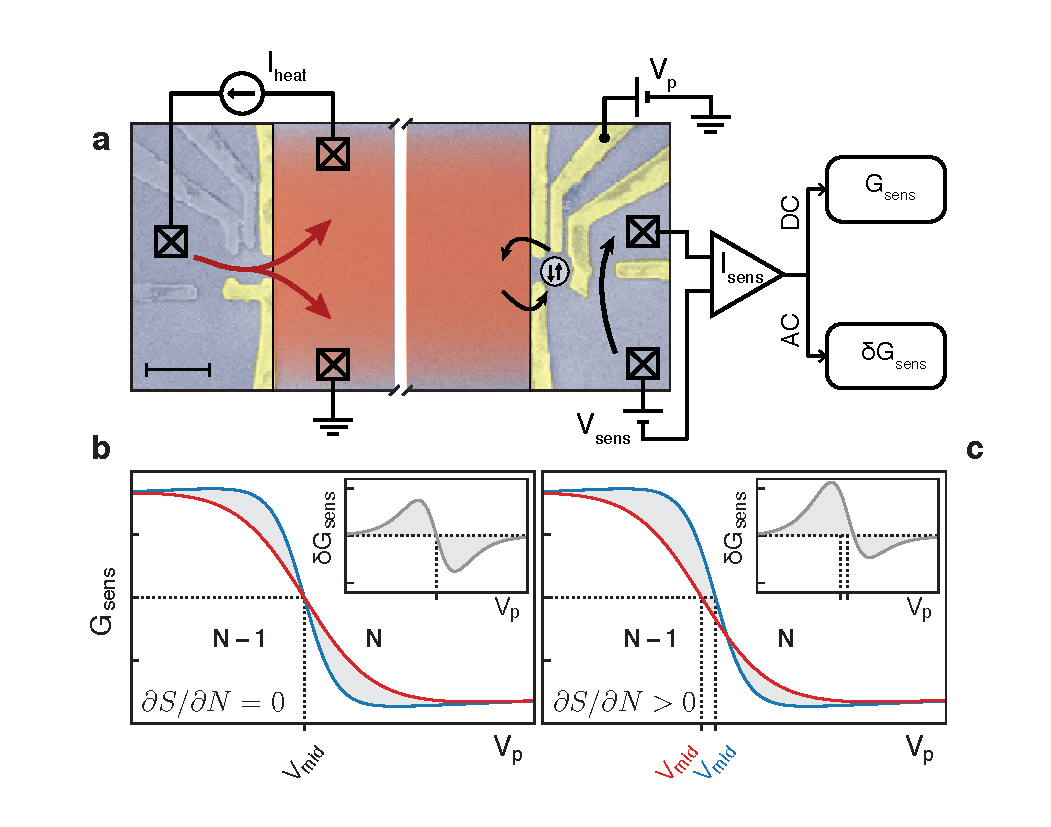
\includegraphics[width=1.0\columnwidth]{../figures/figure_1_annotated.pdf}
        \caption{\label{fig:fig1}(a) Scanning electron micrograph of a device similar to the one measured, showing electrostatic gates (blue) used to define a circuit in the 2D electron gas. Grey gates are unused (grounded). Squares show the locations of ohmic contacts to the 2DEG. An electron reservoir is formed between the parallel gates running vertically down the image. The reservoir can be heated by driving current through the quantum point contact on the left. A 200nm diameter quantum dot is coupled to the right side of the channel. Electrons tunneling between the reservoir and dot are measured with a capacitively-coupled charge sensor. (b) and (c) Charge sensor signal for a single transition from $N-1 \rightarrow N$ electrons at two temperatures ($T_{Red} > T_{Blue}$) showing two possible cases for $\frac{\partial \mu}{\partial T}$.}
\end{figure}

%Entropy can be probed effectively in 3D macroscopic samples via measurements of heat capacity, but the heat capacities of single electrons or quasiparticles are much too small to measure directly; even the 2D sheet of quasiparticles in $\nu = \frac{5}{2}$ fractional quantum Hall samples has a heat capacity that vanishes in comparison to that of the host crystal.  Rather than attempt to resolve such infinitesimal signals, the problem can be avoided by converting changes in entropy to changes in charge \textemdash a quantity that is easily detected at the single particle level.

Our approach is analogous to the milestone of spin-to-charge conversion by which undetectably-small magnetic moments of a single spin were transformed into the presence or absence of an electron charge \cite{Elzerman2004, Ono2004}.  Instead, we perform an entropy-to-charge conversion, making use of the Maxwell relation
%
\begin{align}
\label{eqn:max}
        \left(\frac{\partial \mu}{\partial T}\right)_{p,N} &= -\left(\frac{\partial S}{\partial N}\right)_{p,T}
\end{align}
%
that connects changes in entropy, particle number, and temperature ($S$, $N$, and $T$, respectively) to changes in the chemical potential, $\mu$, a quantity that is simple to measure and control. The fixed pressure condition of Eq.~\ref{eqn:max} is met by working well below the Fermi temperature of the 2DEG, $T_F \sim \SI{5}{\kelvin}$, where degeneracy pressure dominates \cite{Landau1969}.

The Maxwell relation in Eq.~\ref{eqn:max} forms the basis of two theoretical proposals to measure non-Abelian exchange of quasiparticles in the the $\nu = \frac{5}{2}$ state, by detecting changes in the quasiparticle chemical potential with temperature, which are proportional to the entropy derivative, $\frac{\partial S}{\partial N}$ \cite{Cooper2009,Ben-Shach2013}.
%Unlike the $\nu = \frac{5}{2}$ quasiparticles described in the theoretical work, the few-electron quantum dot states investigated here have an entropy that is well-understood from the spin degree of freedom \cite{Tarucha1996, Ciorga2000, Duncan2000, Lindemann2002, Potok2003, Hofmann2016}.  
Applying the language of quantum dots to Eq.~\ref{eqn:max}, the entropy difference between the $N-1$ to $N$ quantum dot ground states ($\Delta S_{N-1\rightarrow N}$ for $\Delta N=1$) is measured through the shift with temperature in the electrochemical potential needed to add the $N$th electron to the dot, $\mu_N$; the gate voltage at which the $N-1$ to $N$ transition is observed shifts proportionally with $\mu_{N}$.
%This shift, $\delta \mu$ as a function of $\delta T$, is the quantity probed directly in the experiment described below. From these measurements the entropies of the first three quantum dot levels are built up, demonstrating a direct entropy measurement is possible on a few-particle system. In the future, the method can be utilized to probe the nature of more exotic systems, such as topologically non-trivial Majorana and other non-Abelian states. 

The mesoscopic circuit shown in Fig.~\ref{fig:fig1}a uses electrostatic gates to realize an electron reservoir (central region; hereafter ``reservoir") in thermal and diffusive equilibrium with a few-electron quantum dot (``dot") coupled to its right side.  The reservoir temperature, $T_{res}$, could be rapidly (up to at least \SI{100}{\hertz}) increased above the mixing chamber temperature, $T_{MC}$, by Joule heating through the QPC (``heater") on the left side.  The occupation of the dot was measured using an adjacent quantum point contact (``charge sensor")\cite{Staring2007, Thierschmann2015} [change these references/add additional].  Applying a more positive voltage to the gate adds the $N$th electron to the dot when $\mu_{N}$ drops below the Fermi level of the reservoir, $E_F$. Figure 1b illustrates such a transition \textemdash a step in the charge sensor conductance \textemdash thermally broadened by the reservoir temperature.  The gate voltage corresponding to midpoint of the transition, $V_{mid}$, marks the electrochemical potential at which the probabilities of finding $N-1$ or $N$ electrons on the dot are equal.  When $\mu_N$ shifts with temperature, $V_{mid}$ also shifts (Fig.~1c); it is this signature that forms the basis of our experiment.%and the $N$th level is occupied half the time. 

The relation between entropy and any temperature-induced shift in $\mu_{N}$ with respect to $E_F$ can also be understood in the language of detailed balance.  The $N$th electron tunnels back and forth between an $N-1$-electron dot and reservoir when there are available states in both the dot and reservoir, that is, when $\mu_{N}$ is within thermal broadening of $E_F$.  The tunnel rates into and out of the dot, $\Gamma_{in}=\Gamma_{N-1\rightarrow N}$ and $\Gamma_{out}=\Gamma_{N\rightarrow N-1}$, depend on degeneracy of the $N-1$ and $N$ ground states.  %Consider the filling of the first electron state, which has a single, unpaired spin-$\frac{1}{2}$ and, therefore, a degeneracy of 2.
Consider, for example, the first electron tunneling into an empty dot: both spin-up and -down states are available.  Tunneling out, the electron (whether spin-up or -down) must tunnel into reservoir states with the same spin, that is, only half of the empty reservoir states are available.  As a result, $\Gamma_{in} = 2\Gamma_{out}$ when $\mu_{N}=E_F$.  Extending this logic to a general case gives the result derived from detailed balance \cite{Gustavsson2009, Beenakker1991}, 
%
\begin{align}
	\Gamma_{in} &=  g_{N} \Gamma f(E_F - \mu_{N}) \nonumber \\
	\Gamma_{out} &= g_{N-1} \Gamma [1 - f(E_F - \mu_{N})] \label{eqn:rates}
\end{align}
%
where $\Gamma$ is a coupling constant, $f$ is the Fermi function, and $g_{N(N-1)}$ is the degeneracy of the $N(N-1)$ electron state.

The equal probability condition for $N-1/N$ at $V_{mid}$ corresponds to  incoming and outgoing rates being equal.  From Eq.~\ref{eqn:rates}$, \Gamma_{in} = \Gamma_{out}$ corresponds to $\mu_{N} = E_F$ as long as $g_{N-1}=g_{N}$, but to $\mu_{N} > E_F$ when $g_{N-1} > g_{N}$ and vice versa.   The ratio $g_{N}/g_{N-1}$ is given by the shift in $V_{mid}$ with temperature, giving $\Delta S_{N-1\rightarrow N}$ via the Boltzmann entropy, $S_{N}=k_{B} \ln{g_N}$. Previous works have explored the relationship between tunnel rates and degeneracy using AFM coupling and time-resolved transport spectroscopy \cite{Cockins2010, Bennett2010, Beckel2014, Hofmann2016}. The approach presented here illustrates the thermodynamic equivalent of the rate measurement, and extends entropy measurements to a wide set of applications where tunneling processes may not be possible to observe in real-time.

%%%%%%%%%%%%%%%%%%%%%%%

%%% figure 2 %%%
\begin{figure}[!]
        \includegraphics[width=1.0\columnwidth]{../figures/figure_2.pdf}
        \caption{\label{fig:fig2}(a) Charge sensor data for $N=0 \rightarrow 1$ at two temperatures set by DC current through the QPC heater. (b) Lock-in measurement of $dg_{sens}$ with $\delta T \sim \SI{60}{\milli\kelvin}$. Fits to $dg_{sens}$ are shown with $\delta$ as a free parameter (solid) and $\delta=0$ (dashed) (c) Transition width, $\Theta$, as a function of mixing chamber temperature. The highlighted region shows roughly where tunnel rates are determined only by temperature broadening. The lever arm $\alpha$ is calculated by fitting a straight line to this region. (d) $\Theta$ as a function of DC current through the QPC heater. Fit is used to convert between $I_{heat}$ and $\delta T$, with $R_{QPC} = \SI{20}{\kilo\ohm}$ (e) Change in entropy as a function of AC current through the QPC heater. Top axis shows corresponding $\delta T$. Right axis shows shift in $\delta V_{mid}$ per unit temperature.}
\end{figure}

%%% device setup %%%
To proceed with the entropy measurement, the quantum dot (Fig.~\ref{fig:fig1}a) was tuned such that the source was weakly tunnel coupled to the reservoir with the drain closed.   The conductance of the charge sensor was tuned to $g_{sens}{\sim}e^2/h$ where it was most sensitive to charge on the dot.  The addition of the first electron to the dot was marked by a decrease in $g_{sens}$ that is well fit by the expected form for a thermally-broadened transition (Fig.~\ref{fig:fig2}a):
%
\begin{align}
\label{eqn:g}
        g_{sens}(V,\Theta) &= G_0 \tanh\left(\frac{V-V_{mid}(\Theta)}{2\Theta}\right)  \\
                        &\quad + G_1\left[V-V_{mid}(\Theta)\right] + G_2 \nonumber
\end{align}
%
where $G_0$ quantifies the sensor sensitivity, $\Theta = \frac{k_B T}{\alpha e}$ is the thermal broadening expressed in units of gate voltage, $\alpha$ is the lever arm $\alpha\equiv\partial \mu_{N}/\partial V_G$, and $G_1$ is determined by the cross capacitance between the charge sensor and plunger gate. With no Joule heating through the heater, $\Theta$ was found to follow $T_{MC}$ down to \SI{<100}{\milli\kelvin} (Fig.~\ref{fig:fig2}b), validating the approximation of thermal broadening used throughout this experiment.

%The transition width, $\Theta$, extracted from fits to Eq.~\ref{eqn:g} follows the mixing chamber temperature, $T_{MC}$, to \SI{<100}{\milli\kelvin} (Fig.~\ref{fig:fig2}b). The assumption of thermally broadened transitions greatly simplifies the data analysis, so $T_{MC}$ is fixed at \SI{100}{\milli\kelvin} for most of this work, using Joule heating to raise $T_{res}$ up to \SI{250}{\milli\kelvin}. Measurements of $\Delta S$ are made at $\delta T_{res} = $ \SI{60}{\milli\kelvin} such that no orbital levels above the ground state were excited.

%%% figs 2c and d%%%
The data in Fig.~\ref{fig:fig2}c, and corresponding fits, offer an example of how $\Delta S_{0\rightarrow 1}$ was measured across the $0 \rightarrow 1$ transition.  A comparison of the curves in Fig.~\ref{fig:fig2}a shows that $g_{sens}$ drops as temperature rises before the midpoint of the transition ($V_G-V_{mid}<0$), whereas $g_{sens}$ is higher in the warmer curve for $V_G-V_{mid}>0$.   Oscillating the reservoir temperature by $\delta T_{res}$ using an AC current through the heater while measuring oscillations in $g_{sens}$ with a lock in amplifier (see Methods) yields the characteristic peak-dip structure seen in Fig.~\ref{fig:fig2}c.  The expected lineshape of such a curve is given by the derivative of Eq.~\ref{eqn:g} with respect to temperature, expressed as $dg_{sens}$ due to a temperature change $\delta T$:
%
\begin{align}
\label{eqn:dg}
        dg_{sens}(V_G, \Theta) &\propto \delta T \left[ \frac{V_G-V_{mid}(\Theta)}{2\Theta} +\delta \right]\times \\
        				      &\quad\cosh^{-2}\left(\frac{V_G-V_{mid}(\Theta)}{2\Theta}\right) + const. \nonumber
\end{align}
%
where $\delta=\frac{\partial V_{mid}}{\partial \Theta}$. Using the lever arm to convert $V_{mid}$ to electrochemical potential, $\delta$ is simply the change in entropy (scaled by $k_B$) through Eq.~\ref{eqn:max}:
%
\begin{align}
\label{eqn:delta}
        \delta &= \frac{\partial V_{mid}}{\partial \Theta} = 
        \frac{1}{k_B} \frac{\partial \mu}{\partial T} = 
        -\frac{1}{k_B} \Delta S_{N-1\rightarrow N}
\end{align}
%

From Eqs.~\ref{eqn:dg} and \ref{eqn:delta}, $dg_{sens}(V_G)$ would be perfectly antisymmetric around $V_{mid}$ if $\Delta S_{N-1\rightarrow N}$ were zero.  The best fit of Eqs.~\ref{eqn:dg} and \ref{eqn:delta} to the data in Fig.~\ref{fig:fig2}c yields $\Delta S_{0\rightarrow 1}=0.71\times k_B$.  Indeed, this is what would be expected for the $0 \rightarrow 1$ electron transition at zero magnetic field: $S_0$ for the empty state should be $k_B \ln{1}=0$ whereas for the spin degenerate 1-electron state one expects $S_1=k_B\ln{2}$, giving $\Delta S_{0\rightarrow 1}\equiv S_1 = S_0 =k_B\ln{2}$. Fig.~\ref{fig:fig2}e shows that $\Delta S$,  determined from fits to data analogous to Fig.~\ref{fig:fig2}c, remains constant over a range of $\delta T_{res}$ ($I^{AC}_{Heat}$).  Although the extracted $\delta$ can be converted to gate-voltage-per-temperature units using a value for $\alpha$ measured separately (right axis of Fig.~\ref{fig:fig2}e), the entropy itself, $\Delta S$, is determined directly from the fit to $dg_{sens}$ without any additional calibration, and without knowing the precise value of $\delta T_{res}$.

%%% figure 3 %%%
\begin{figure}
        \includegraphics[width=1.0\columnwidth]{../figures/figure_3.pdf}
        \caption{\label{fig:fig3}(a) Change in entropy, determined from $dg_{sens}$ fits at varying parallel magnetic field. The $N=0 \rightarrow 1$ and $2 \rightarrow 3$ data are overlaid here to show the similar behavior of these states at low field. (b) and (c) show characteristic $dg_{sens}$ traces from which the data in (c) were extracted. These data points are show as large markers in (c). (e) Bias spectroscopy data for $N=0 \rightarrow 1$ transition. Dashed line at $V_{SD}$ = \SI{700}{\micro\electronvolt} shows where data in (f) are taken. (f) Fixed bias data showing fits to Zeeman splitting of the ground state (dashed lines) from which $g = -0.44$ is extracted.}
\end{figure}

Confirmation that the measured $\Delta S$ derives from spin degeneracy can be seen in its evolution with in-plane magnetic field, $B_\parallel$. Figure \ref{fig:fig3}a compares $\Delta S(B_\parallel)$ for the 0-1 and 2-3 electron transitions.  The 2-electron ground state is a spin singlet, while the 3-electron ground state adds an additional unpaired electron, so both $\Delta S_{0 \rightarrow 1}$ and $\Delta S_{2 \rightarrow 3}$ are expected to correspond to transitions from total spin zero to total spin one-half.
%One expects identical field-dependent behaviors for $\Delta S_{0\rightarrow 1}$ and $\Delta S_{2\rightarrow 3}$ as long as $g \mu_{B} B_\parallel$ is less than the excited state energies.
The entropies of the 1- and 3-electron states are suppressed when Zeeman splitting lifts the spin degeneracy of the unpaired electron. This behavior is described by the Gibbs entropy for a two-level system:
%
\begin{align}
\label{eqn:gibbs}
        S &= k_B \sum_{i=\pm} p_{i}(B_\parallel, T) \ln{ p_{i}(B_\parallel,T) }
\end{align}
%
where $p_{\pm}(B_\parallel, T) = (1+ e^{\mp \frac{g\mu_B B_{\parallel}}{k_B T}})^{-1}$ are the probabilities for the unpaired electron to be in the spin up/down states at a given field and temperature. Fits to Eq.~\ref{eqn:gibbs} are shown in Fig.~\ref{fig:fig3}a for both transitions, allowing for peak height and the ratio $g/T_{res}$ as free parameters.

The entropy measurements yield $\Delta S_{0 \rightarrow 1}=0.93\times k_B \ln{2}$ and $\Delta S_{2 \rightarrow 3}=0.98\times k_B \ln{2}$ at zero magnetic field, collapsing to zero at high field where spin degeneracy is broken.  At a qualitative level, Figs.~\ref{fig:fig3}b and c show $dg_{sens}$ crossover from asymmetric to antisymmetric as $\Delta S$ goes to zero at high field. Using $T_{res} = \SI{130}{\milli\kelvin}$, midway between the low ($T_{MC}$) and high ($T_{MC}+\delta T$) points of the temperature oscillation, yields $g=-0.39$ and $g=-0.40$ for the $0\rightarrow 1$ and $2\rightarrow 3$ transitions, respectively. These are consistent with $g=-0.44$ expected for GaAs and measured via bias spectroscopy in Fig.~\ref{fig:fig3}e.

%%% figure 4 %%%
\begin{figure}
        \includegraphics[width=1.0\columnwidth]{../figures/figure_4.pdf}
        \caption{\label{fig:fig4}(c) Change in entropy, extracted from $dg_{sens}$ fits at varying parallel field. Dashed line shows fit to Eq.~\ref{eqn:gibbs} (b), (c), and (d) show characteristic $dg_{sens}$ traces from which the data in (c) were extracted. These data points are show as large markers in (c). (e) Bias spectroscopy data for the $N=1 \rightarrow 2$ transition. Singlet-triplet splitting is \SI{316}{\micro\electronvolt}. Dashed line at $V_{SD}$ = \SI{1250}{\micro\electronvolt} shows where data in (f) are taken. (f) Fixed bias data in parallel field. Triplet level is split into $T_+$, $T_0$, and $T_{-}$ (not visible). At \SI[input-protect-tokens]{\sim 9}{\tesla} $T_+$ becomes degenerate with $S$. $g=-0.40$ is determined using $T_0$ and $T_+$ fits (dashed).}
\end{figure}

The $1\rightarrow 2$ transition (Fig.~\ref{fig:fig4}a) can be understood as the inverse of Fig \ref{fig:fig3}a for $B_\parallel < \SI{5}{\tesla}$.  There, the 2-electron ground state remains a spin singlet ($S_2=0$) while the 1-electron ground state entropy goes from $k_B\ln{2}$ to zero due to Zeeman splitting. At higher field, the 1-electron ground state remains non-degenerate ($S_1=0$) while the 2-electron ground state becomes two-fold degenerate where the spin singlet ($S$) and triplet ($T_+$) states cross. The singlet-triplet crossing is seen clearly around at \SI{9}{\tesla} in bias spectroscopy data for the $1\rightarrow 2$ transition (Fig.~\ref{fig:fig4}e). 

The field-dependent entropy measurement for the 1-2 transition can again be fit using Eq.~\ref{eqn:gibbs}, with probabilities as before for the 1-electron states and $p_{S/T}(B_\parallel, T) = (1+ e^{\mp \frac{g\mu_B B_\parallel - \Delta_{ST}}{k_B T}})^{-1}$ for the 2-electron states, where $\Delta_{ST}$ is the singlet-triplet splitting at zero field. The fit allows for an offset from $\Delta S=0$, away from the degenerate points, to compensate for non-linearities in the charge sensor. From the fit we find the entropies at the two-fold degenerate points, $B=0$ and \SI{9}{\tesla}, are again within 5\% of the expected values, $\mp k_B \ln{2}$. The extracted value of $g = 0.39$ from the low-field peak agrees well with the fit in Fig.~\ref{fig:fig3}a. At the high-field singlet-triplet degeneracy we find $g = 0.59$. This unexpectedly high g-factor can be explained by a shifting of the $T_{0}$ state with magnetic field, as seen in Fig.~\ref{fig:fig4}f and previous work \cite{Szafran2004}. The high quality of the Gibbs entropy fit confirms $\Delta S$ and illustrates a tunable degeneracy in the system.

%%% conclusion %%%
In conclusion, we show that the entropy of few-particle states in mesoscopic devices can be measured directly.  Using the well-understood spin degeneracy of  few-electron ground states states in a GaAs quantum dot for calibration, the entropy can be quantified within 5\% of the expected $\pm k_B\ln{2}$.  Future work may take advantage of this strategy to look for thermodynamic signatures of non-trival electron and quasiparticle states, eliminating the uncertainty found in typical transport data.

\paragraph*{Methods} The device was built on a AlGaAs/GaAs heterostructure, hosting a 2D electron gas with density and mobility at \SI{300}{\milli\kelvin} (determined on a separate chip) of \SI{2.42e11}{\per\square\centi\metre} and \SI[per-mode=symbol]{2.56e6}{\square\centi\metre\per\volt\per\second}.   Mesas and NiAuGe ohmic contacts to the 2DEG were defined by standard photolithography techniques, followed by atomic layer deposition of \SI{10}{\nano\metre} $\mathrm{HfO_2}$ to improve the gating stability to the device. Fine gate structures, including the \SI{200}{\nano\metre} diameter quantum dots, were defined by electron beam lithography and deposition of \SI{20}{\nano\metre} Ti/Au. The measurement was carried out in an dilution refrigerator with a base temperature of \SI{14}{\milli\kelvin}.

The conductance of the charge sensor was measured at a DC voltage bias of \SI{200}{\micro\volt}, with the current read out directly or fed into a lockin amplifier.  The temperature of the reservoir could be raised above $T_{MC}$ (to $T_{MC} + \delta T$) using AC or DC current biased through the left (heater) QPC, which was gate-tuned to \SI{20}{\kilo\ohm}. A calibration for $\delta T$ in this mode, using DC current bias $\alpha$ as measured in Fig.~\ref{fig:fig2}b, can be seen in Fig.~\ref{fig:fig2}c. Applying AC current at $f_{Heat} =$ \SI{48.7}{\hertz} yields oscillations in $T_{res}$ at $2f_{heat}$; to leading order $\delta T_{res} \sim P \sim \cos(2 \times (2 \pi f_{heat}) \times t)$. Variations in $g_{sens}$ with $\delta T$ are captured with a lockin amplifier measuring $g_{sens}$ oscillations at at the second harmonic of $f_{heat}$.

The transition width, $\Theta$, extracted from fits to Eq.~\ref{eqn:g} was found to follow the mixing chamber temperature, $T_{MC}$, to \SI{<100}{\milli\kelvin} (Fig.~\ref{fig:fig2}b). The assumption of thermally broadened transitions greatly simplifies the data analysis, so $T_{MC}$ is fixed at \SI{100}{\milli\kelvin} for most of this work, using Joule heating to raise $T_{res}$ up to \SI{250}{\milli\kelvin}. Measurements of $\Delta S$ are made at $\delta T_{res} = $ \SI{60}{\milli\kelvin} such that no orbital levels above the ground state were excited.

%\acknowledgments

\bibliography{qdentropy}{}
\bibliographystyle{apsrev4-1}

\end{document}